\documentclass[11pt,a4paper]{article}
\usepackage[hmargin=2.4cm,vmargin=2.2cm]{geometry}
\usepackage[T1]{fontenc}
\usepackage{lmodern}
\usepackage{microtype}
\usepackage{amsmath}
\usepackage{booktabs}
\usepackage{tabularx}
\usepackage{caption}
\usepackage{subcaption}
\usepackage{placeins}
\usepackage{tikz}
\usepackage{pgfplots}
\usepackage[hidelinks]{hyperref}
\pgfplotsset{compat=1.17}
\definecolor{cA}{HTML}{2A78D6}
\definecolor{cB}{HTML}{EB6834}
\captionsetup{font=small,labelfont=bf}
\captionsetup[sub]{font=small}
\setlength{\parindent}{0pt}
\setlength{\parskip}{0.45em}
\makeatletter\setlength{\@fptop}{0pt}\makeatother
\newcolumntype{L}{>{\raggedright\arraybackslash}X}
\newcommand{\tabnote}[1]{\par\smallskip\parbox{\linewidth}{\footnotesize #1}}
\pgfplotsset{
  esaxis/.style={width=\linewidth, height=5.0cm, ymajorgrids, grid style={gray!25},
    tick label style={font=\scriptsize}, label style={font=\scriptsize},
    xticklabel style={/pgf/number format/.cd, fixed, precision=0, 1000 sep={}},
    legend style={font=\scriptsize, draw=none, at={(0.5,-0.16)}, anchor=north, legend columns=1},
    legend cell align=left},
  ci/.style={only marks, mark size=1.4pt, error bars/y dir=both, error bars/y explicit,
    error bars/error bar style={line width=0.5pt}}
}

\begin{document}

{\Large\bfseries What is urban density worth to young adults?\par}
\vspace{0.2em}
{\large Evidence from the COVID-19 closures in London and England and Wales\par}
\vspace{0.6em}
{\small Paper 7, Regional Economics and Policy, supervision 3, Part A \hfill Affan, November 2026\par}
\vspace{0.3em}
\hrule
\vspace{0.4em}

%======================================================================
\section{The question}
%======================================================================

People and firms locate in large cities despite higher housing and land costs because of agglomeration benefits, which for producers include larger labour markets, shared suppliers and the spread of ideas, and for consumers include access to a wider range of goods and services. Part of the benefit to consumers is a preference for variety in consumption, and a young adult in London can reach theatres, galleries, live music venues, bars, nightclubs and restaurants in far greater number and range than a young adult in Stirling for instance. In Glaeser's account of the consumer city this difference is central to urban growth. However, the value of the preference is difficult to measure, because residents pay for every benefit of density through the same rent, and the specific share of that rent paid for their preference for variety in consumption is unobserved.

During the COVID-19 closures access to this variety was removed for about a year and restored on known dates. Most hospitality and leisure venues in England closed in late March 2020, reopened in stages from July 2020, closed again over the autumn and winter and reopened for indoor service on 17 May 2021. Before the closures a resident of Westminster, the London borough with the most hospitality and leisure establishments per resident, had far more venues within reach than a resident of Barking and Dagenham, the borough with the fewest, and paid a higher rent partly for that access. During the closures both residents had almost no venues open within reach, whilst the Westminster resident continued to pay the higher rent. When the first lockdown was announced, some residents of large cities moved elsewhere, often to be closer to family. A young adult who lives in London gives up proximity to family in exchange for the consumption and employment available in the city, so when consumption variety was removed and work moved online, the value of staying fell, and the number of young adults who left is a measure of how much that variety and access to employment were worth to them. Their return after the reopening is a measure of the same value from the other direction.

London boroughs were therefore ranked by their hospitality, arts and leisure establishments, public and private, per resident in 2019, called amenity density here, from 2.49 per 1,000 residents in Barking and Dagenham to 32.75 in Westminster, and migration into and out of each borough was followed through the closures and the reopening. Young adults mostly rent and have the lowest moving costs, so their net migration is compared with that of older residents of the same borough and year, whereby every shock common to all ages in a borough, including local housing costs and employment, is absorbed. The same design is extended to 316 local authorities and, within them, 7,262 small areas (MSOAs) of England and Wales, with ONS net migration by single year of age for the years to June 2016 to 2025.

After the reopening it can also be tested whether young residents returned to dense places once the variety of consumption there was restored. If young adults left because variety was removed, dense places should have regained them once it returned, and such a recovery would strengthen the reading of the 2020 outflow as a valuation of variety. Davis and Weinstein found that Japanese cities returned to their pre-war positions within about fifteen years of the Allied bombing, consistent with populations pinned down by fundamentals, whilst Monte, Porcher and Rossi-Hansberg find that commuting in the largest US cities settled at about 60 per cent of its pre-pandemic level. The recovery test is applied to residents aged 25 to 34, who are mostly beyond university age, so that the result is free of the movement of students between term-time and home addresses.

%======================================================================
\section{Findings}
%======================================================================

\subsection*{1. Young adults left dense places when their consumption value closed and returned when it reopened}

In London a borough with one standard deviation higher amenity density lost 5.2 net young residents per 1,000 relative to older residents in the year to June 2020 ($p = 0.002$), about a quarter of the average net inflow of young adults into a borough before 2020, and gained 8.1 in 2022, a reversal of 13.3 per 1,000 (Figure~\ref{fig:main}a). Across England and Wales, with population-weighted access to food venues as the measure of density, the 2020 coefficient is $-5.5$ and the reversal $+11.1$ per 1,000 with teleworkability, the share of jobs that can be done from home, and garden access held fixed, both with $p < 0.001$, and the 2020 and 2022 coefficients lie 5.3 below and 9.4 above the pre-2020 trend (Figure~\ref{fig:main}b). The response is therefore a measure of the value young adults place on density beyond living space and remote working, taken from behaviour within places and years, whereas in cross-sectional rents that value is combined with every other attribute of location. There are, however, three limits to this measure, namely that access to food venues was chosen after a registered test, one whose decision rule was fixed in advance in a pre-analysis plan, in which the reversal with venues per resident as the measure was $-1.5$ ($p = 0.191$) and tourist districts such as the Cotswolds and South Hams ranked among the densest, that the 2022 return lasted one year, with relative outflows resuming from 2023 as interest rates and central rents rose, and that access is built from the Food Standards Agency register as held in October 2026, so venues that opened or closed between 2019 and 2026 enter a measure intended for 2019. Across the 316 districts the logged 2026 register counts of restaurants and cafes, takeaways and pubs and bars correlate at 0.93 to 0.96 with the 2019 Business Counts of the same venue types, and in the Census and venue-mix designs of Table~\ref{tab:registered} the estimates with a 2019 OpenStreetMap measure of access are $-6.27$ and $-0.96$, against $-6.18$ and $-1.28$ with the register, although the triple difference itself has not been re-estimated with a 2019 source.

\begin{figure}[htbp]
\centering
\begin{subfigure}[t]{0.49\linewidth}
\centering
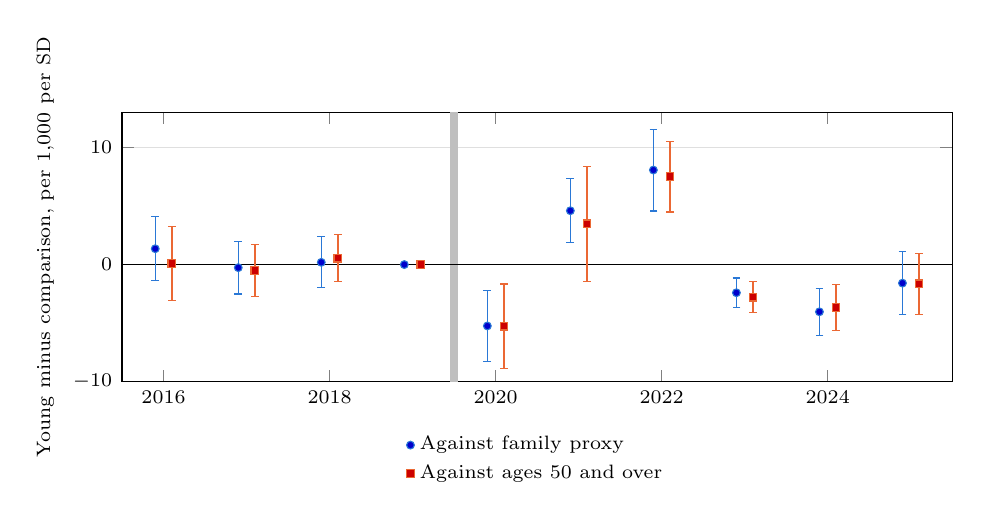
\begin{tikzpicture}
\begin{axis}[esaxis, xmin=2015.5, xmax=2025.5, ymin=-10, ymax=13, xtick={2016,2018,...,2024},
  ylabel={Young minus comparison, per 1,000 per SD}]
\addplot[gray!50, line width=3pt, forget plot] coordinates {(2019.5,-10) (2019.5,13)};
\addplot[black, thin, forget plot] coordinates {(2015.5,0) (2025.5,0)};
\addplot+[ci, color=cA, mark=*] coordinates {(2015.9,1.3543) +- (0,2.7311) (2016.9,-0.2629) +- (0,2.2555) (2017.9,0.1907) +- (0,2.1706) (2018.9,0.0000) +- (0,0.0000) (2019.9,-5.2440) +- (0,3.0289) (2020.9,4.6011) +- (0,2.7411) (2021.9,8.0780) +- (0,3.5021) (2022.9,-2.4070) +- (0,1.2632) (2023.9,-4.0359) +- (0,2.0229) (2024.9,-1.5850) +- (0,2.7002)};
\addlegendentry{Against family proxy}
\addplot+[ci, color=cB, mark=square*] coordinates {(2016.1,0.0738) +- (0,3.1724) (2017.1,-0.5291) +- (0,2.2353) (2018.1,0.5498) +- (0,2.0314) (2019.1,0.0000) +- (0,0.0000) (2020.1,-5.2578) +- (0,3.5966) (2021.1,3.4749) +- (0,4.9033) (2022.1,7.5048) +- (0,3.0131) (2023.1,-2.7792) +- (0,1.3108) (2024.1,-3.6704) +- (0,1.9462) (2025.1,-1.6526) +- (0,2.6021)};
\addlegendentry{Against ages 50 and over}
\end{axis}
\end{tikzpicture}
\caption{London, 32 boroughs, log amenity density}
\end{subfigure}\hfill
\begin{subfigure}[t]{0.49\linewidth}
\centering
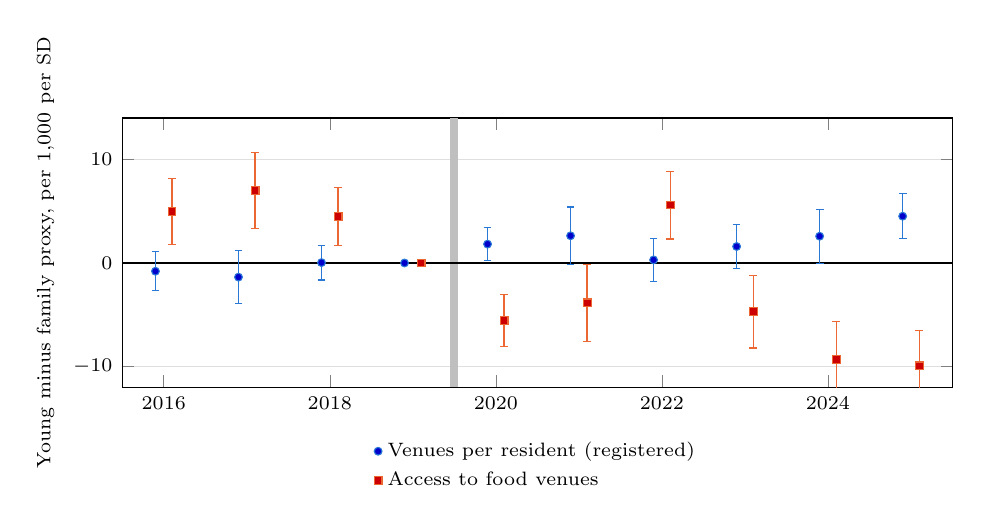
\begin{tikzpicture}
\begin{axis}[esaxis, xmin=2015.5, xmax=2025.5, ymin=-12, ymax=14, xtick={2016,2018,...,2024},
  ylabel={Young minus family proxy, per 1,000 per SD}]
\addplot[gray!50, line width=3pt, forget plot] coordinates {(2019.5,-12) (2019.5,14)};
\addplot[black, thin, forget plot] coordinates {(2015.5,0) (2025.5,0)};
\addplot+[ci, color=cA, mark=*] coordinates {(2015.9,-0.7944) +- (0,1.8926) (2016.9,-1.3634) +- (0,2.5829) (2017.9,0.0374) +- (0,1.6859) (2018.9,0.0000) +- (0,0.0000) (2019.9,1.8231) +- (0,1.6011) (2020.9,2.6285) +- (0,2.7787) (2021.9,0.2972) +- (0,2.0943) (2022.9,1.5926) +- (0,2.0864) (2023.9,2.5834) +- (0,2.5916) (2024.9,4.5190) +- (0,2.1843)};
\addlegendentry{Venues per resident (registered)}
\addplot+[ci, color=cB, mark=square*] coordinates {(2016.1,4.9908) +- (0,3.1896) (2017.1,7.0276) +- (0,3.6623) (2018.1,4.4729) +- (0,2.8067) (2019.1,0.0000) +- (0,0.0000) (2020.1,-5.5368) +- (0,2.4960) (2021.1,-3.8519) +- (0,3.7110) (2022.1,5.5983) +- (0,3.2780) (2023.1,-4.6938) +- (0,3.5221) (2024.1,-9.3528) +- (0,3.7004) (2025.1,-9.9436) +- (0,3.4052)};
\addlegendentry{Access to food venues}
\end{axis}
\end{tikzpicture}
\caption{England and Wales, 316 districts}
\end{subfigure}
\caption{Net migration of residents aged 20 to 29 relative to older residents of the same place, per standard deviation of density, by year ending June. Triple-difference coefficients from equation~(\ref{eq:ddd}) relative to 2019, with 95 per cent confidence intervals clustered by place. In panel (b) teleworkability and garden access are held fixed, and the access measure was chosen after the registered results.}\label{fig:main}
\end{figure}

\subsection*{2. The residential value of density in Britain arrives as one bundle}

Consumption variety and the other benefits of density move together so closely in Britain that the response of young adults to one is also a response to the others. Across districts access to food venues correlates at 0.90 with job density and 0.89 with resident density, and across London boroughs amenity density correlates at 0.82 with teleworkability and $-0.73$ with garden access, so that within London the 2020 coefficient is $+2.1$ ($p = 0.387$) once both are held fixed. Four designs were built to separate variety, with variation across boroughs, across districts in venues per resident, in extra local closure days under the tier system of late 2020 and within districts in the mix of venue types that closed, and in each the variation in lost variety moved with density itself or with a neighbourhood trend already under way before 2020 (Table~\ref{tab:designs}). Puga's bundling problem for firms thereby has a household counterpart, and British estimates of the consumer city from cross-sections or annual migration are estimates of the whole bundle.

The closure calendar was coded from 42 rules in the coronavirus regulations for England and Wales, and from it the composition of that variety can be measured. Restaurants and cafes make up 52 per cent of the venues within reach of the average neighbourhood, takeaways 26 per cent and pubs and bars 20 per cent, whilst cinemas, theatres, gyms and nightclubs together make up about 2 per cent. Takeaways stayed open throughout, so the share of local variety lost in a neighbourhood fell as its takeaway share rose, with a correlation of $-0.92$, and the variety near British homes is largely food and drink. For town-centre, licensing and night-time economy policy, which is directed at one element of the bundle, the response to losing the whole bundle, about 5 net young residents per 1,000 per standard deviation of access within a year, is an upper scale for what venue policy alone can achieve.

\subsection*{3. Dense places regained their young residents, with full recovery outside London}

In the test of Davis and Weinstein the change in an area's young population during the closures, from 2019 to 2021, is related to its change afterwards, from 2021 to 2024, and a coefficient of $-1$ corresponds to full recovery and 0 to a lasting shift. Part of the change from 2019 to 2021 in small areas reflects measurement error and causes unrelated to the closures, so that change is predicted from each area's access to food venues and only the part linked to access is used. On this basis small areas that lost more residents aged 25 to 34 had regained about half of the loss by 2024, with a coefficient of $-0.51$ across 7,262 MSOAs and a 95 per cent interval from $-1.11$ to $0.10$ that contains both benchmarks, so the registered verdict is inconclusive (Figure~\ref{fig:rec}). Two further readings, registered outside the decision rule, lie closer to full recovery. When the same test is run on the years 2015 to 2019, before the pandemic, the coefficient is $+1.28$, so access was already related to young-adult growth in ordinary years, and relative to that ordinary pattern the recovery coefficient is lower by 1.79 (interval $-2.54$ to $-1.04$), a reading that is valid if the pre-2020 pattern would have continued unchanged. Outside London the coefficient is $-0.71$ (interval $-1.37$ to $-0.05$), a reading of full recovery. Outside London, dense places therefore recovered their young residents in the way Davis and Weinstein found for bombed Japanese cities, in contrast to the tipping that Monte, Porcher and Rossi-Hansberg find for commuting in the largest US cities, with the limit that in London, the British counterpart of those cities, the first-stage F of 1.3 is too weak for a test.

\subsection*{4. Methodology with the help of AI}

The research was carried out with Claude Code, an LLM coding assistant, under a division of labour in which the questions and decisions were mine and the data work was delegated. I set the question, suggested each source, measure of density, comparison group and test, and interpreted each result, and Claude Code wrote and ran the Python for each step and reported the output back for the next decision. The delegated work included downloading the data from the ONS, Nomis, the Food Standards Agency and OpenStreetMap, coding the 42 closure rules from the regulations on legislation.gov.uk, building the access and variety-days-lost measures, and estimating the triple differences with the wild cluster bootstrap.

To ensure that every result could be checked and that each verdict was fixed before its result was seen, three safeguards were enforced, namely (i) the decision rules for the national, venue-mix and recovery tests were written into pre-analysis plans and fixed with a SHA-256 checksum, a digital fingerprint that changes if the file is edited, before those tests were run (Table~\ref{tab:registered}), (ii) every judgement call, departure from a plan and blocked source was recorded in a notes file as it arose, with analyses chosen after the registered results labelled as such, and (iii) each closure rule was checked against the text of its regulation, and the national estimation code was checked by reproducing the London estimates exactly.

The code, cleaned data, notes and pre-analysis plans are available on the \texttt{my-supervision} branch at \url{https://github.com/dziyaulaffan/land-economy-supervision/tree/my-supervision}, with the sources, the steps to reproduce each result and the decision log set out in the \texttt{templates} folder and the scripts and data in the \texttt{london-variety} folder.
%======================================================================
\section{Methodology}
%======================================================================

\subsection{Data}

The London units are the 32 boroughs, excluding the City of London, whose 8,765 residents in mid-2019 shared 1,805 hospitality and leisure units. The national units are 316 of the 318 local authority districts of England and Wales on April 2023 boundaries, excluding the City of London and the Isles of Scilly, and the 7,262 MSOAs of the 2021 Census that lie within those districts.\footnote{England and Wales contain 7,264 MSOAs, and the City of London and the Isles of Scilly each contain one, which is dropped with its district, so the recovery design is estimated on 7,262 MSOAs in 316 districts. The venue-mix design is restricted to the 6,856 MSOAs of England, of which 57 have no Census 2021 inflows at ages 25 to 34, because age detail for those areas was withheld under ONS disclosure rules or published only in coarse bands, and 2 are the MSOAs of the City of London and the Isles of Scilly, leaving 6,797 MSOAs in 294 districts.}

\begin{table}[htbp]
\centering
\caption{Data sources}\label{tab:sources}
\small
\begin{tabularx}{\linewidth}{@{}>{\raggedright\arraybackslash}p{3.6cm}L>{\raggedright\arraybackslash}p{3.3cm}@{}}
\toprule
Measure & Source & Coverage \\
\midrule
Hospitality and leisure units & ONS UK Business Counts, local units in SIC divisions 55, 56 and 90 to 93 & March 2019; boroughs, districts, MSOAs \\
Food venues & Food Standards Agency Food Hygiene Rating Scheme register & Snapshot of October 2026 \\
Cinemas, theatres, gyms, nightclubs & OpenStreetMap & 2019 \\
Internal migration & ONS internal migration estimates, origin by destination by single year of age & Years to June 2015 to 2025 \\
Population, districts & ONS mid-year estimates, rebased to Census 2021 & Mid-2011 to mid-2025 \\
Population, small areas & ONS small area population estimates, single year of age & Mid-2011 to mid-2024 \\
Census migration & Address one year before the census & 2001, 2011, 2021; MSOAs \\
Closure rules & Coronavirus regulations for England and Wales, legislation.gov.uk & March 2020 to December 2021 \\
Case rates and mobility & UK Health Security Agency; Google Community Mobility Reports & 2020 to 2022 \\
Jobs & ONS Business Register and Employment Survey & 2019 \\
Controls & Census 2011 and 2021; ONS garden access; ONS homeworking score & 2011, 2020, 2021 \\
\bottomrule
\end{tabularx}
\end{table}

\subsection{Measures}

Amenity density, the London measure and the registered national measure, is built from the number of hospitality and leisure local units per 1,000 residents in 2019, a rate that ranges from 2.49 in Barking and Dagenham to 32.75 in Westminster, and it enters the regressions as the logarithm of that rate, standardised across units. Access to food venues for MSOA $m$ is the sum of the venues $j$ in the hygiene register, each discounted by distance $d_{mj}$ in kilometres from the MSOA's population-weighted centroid,
\begin{equation}\label{eq:access}
A_m = \sum_j \exp(-d_{mj}/1.5),
\end{equation}
and the district measure is the population-weighted mean of $A_m$ over a district's MSOAs, entered as a standardised logarithm. Variety-days lost is a weighted mean of the share of days $s_{lv}$ each of seven venue types $v$ was closed in district $l$ from 23 March 2020 to 22 March 2021, with access to each type as the weight,
\begin{equation}\label{eq:vdl}
\mathrm{VDL}_m = 365 \times \frac{\sum_v A_{mv} \, s_{lv}}{\sum_v A_{mv}},
\end{equation}
with 1 for closure to the public, 0.5 for partial closure such as outdoor service only and 0 for opening. The migration outcome is net migration between a place and the rest of the United Kingdom per 1,000 mid-2019 residents of the age group, with a family proxy combining ages 0 to 15 and 30 to 49.

\subsection{Triple difference}

In a triple difference the change in net migration relative to 2019 is compared along three dimensions, namely between years, between denser and less dense places, and between young adults and older residents of the same place and year, so that any shock common to all ages in a place, such as a change in local rents or employment, cancels out and only the change specific to young adults in denser places remains. For place $b$, age group $g$ and year ending in June $t$,
\begin{equation}\label{eq:ddd}
y_{bgt} = \alpha_{bt} + \gamma_{gt} + \delta_{bg} + \sum_{k \neq 2019} \theta_k \, D_b \, Y_g \, \mathbf{1}[t = k] + \varepsilon_{bgt},
\end{equation}
where $Y_g$ marks residents aged 20 to 29, $D_b$ is the standardised density measure, and $\alpha_{bt}$, $\gamma_{gt}$ and $\delta_{bg}$ are place-by-year, group-by-year and place-by-group fixed effects. With place-by-year effects every shock common to all ages in a place and year is absorbed, so $\theta_k$ is the additional change relative to 2019 for young adults in a place one standard deviation denser. The reversal is $\theta_{2022} - \theta_{2020}$, since the year to June 2022 is the first full year after reopening. In the national specification teleworkability, garden access and region effects are each interacted with $Y_g$ and year. Standard errors are clustered by place, and p-values are computed with the wild cluster restricted bootstrap with Rademacher weights and 9,999 replications. The first year of the sample is 2016, chosen after a positive 2015 coefficient was seen in London.

\begin{table}[htbp]
\centering
\caption{Triple-difference estimates, ages 20 to 29 against the family proxy}\label{tab:ddd}
\small
\begin{tabularx}{\linewidth}{@{}Lccc@{}}
\toprule
 & $\theta_{2020}$ & $\theta_{2022}$ & $\theta_{2022} - \theta_{2020}$ \\
\midrule
\multicolumn{4}{@{}l}{\textit{London, 32 boroughs, amenity density}} \\
\quad No controls & $-5.24$ (0.002) & $8.08$ ($<0.001$) & $13.32$ ($<0.001$) \\
\quad Teleworkability and garden access & $2.08$ (0.387) & $3.86$ (0.150) & $1.78$ (0.653) \\
\multicolumn{4}{@{}l}{\textit{England and Wales, 316 districts, with teleworkability and garden access}} \\
\quad Venues per resident (registered) & $1.82$ (0.030) & $0.30$ (0.785) & $-1.53$ (0.191) \\
\quad Access to food venues & $-5.54$ ($<0.001$) & $5.60$ (0.001) & $11.14$ ($<0.001$) \\
\quad Access, outside London (284) & $-5.19$ ($<0.001$) & $5.40$ (0.002) & $10.59$ ($<0.001$) \\
\quad Access, job and resident density held fixed & $-5.47$ (0.024) & $5.14$ (0.052) & $10.61$ ($<0.001$) \\
\quad Access, deviation from pre-2020 linear trend & $-5.28$ ($<0.001$) & $9.36$ ($<0.001$) & \\
\bottomrule
\end{tabularx}
\tabnote{Net moves per 1,000 group residents per standard deviation of density, with wild cluster bootstrap p-values in brackets. All rows with access to food venues were chosen after the registered results were known. Against residents aged 50 and over the London coefficients are $-5.26$ in 2020 and $+7.50$ in 2022.}
\end{table}

\FloatBarrier
\subsection{Designs for separating variety}

In the venue-mix design the change in movers aged 25 to 34 per 1,000 residents between the 2011 and 2021 Censuses is regressed on variety-days lost, with district fixed effects and nine controls, among them total access, population and job density, teleworkability and garden access, so the coefficient is identified from differences in the mix of venue types within districts. Under its registered rule, support was defined as a negative headline with $p < 0.05$, a placebo on the 2001 to 2011 change with $p \ge 0.10$ and at most half the size of the headline, and a smaller response for ages 50 and over. Before any outcome was opened, 67 per cent of the variance of the treatment was accounted for by district effects and the controls, and the residual standard deviation was 10.4 days, against a stopping threshold of 2.

\begin{table}[htbp]
\centering
\caption{Four designs for separating consumption variety}
\renewcommand{\arraystretch}{1.15}\label{tab:designs}
\footnotesize
\begin{tabularx}{\linewidth}{@{}>{\raggedright\arraybackslash}p{2.7cm}>{\raggedright\arraybackslash}p{3.4cm}>{\raggedright\arraybackslash}p{3.0cm}L@{}}
\toprule
Design & Separating variation & Headline (p-value) & Limit \\
\midrule
London boroughs, unregistered & Amenity density with teleworkability and garden controls, 32 boroughs & 2020 coefficient $+2.08$ (0.387) with both controls & Amenity density correlates at 0.82 and $-0.73$ with the two controls \\
National triple difference, national plan & Venues per resident, 316 districts & Reversal $-1.53$ (0.191) & The measure is highest in tourist areas, and the access measures correlate at about 0.9 with density \\
Tier closures, national plan & Extra closure days beyond national lockdowns, 316 districts & Interaction with density $+0.24$ (0.847) & With annual totals the first stage across districts is weak (0.581), and the days were set by case rates \\
Venue mix, venue-mix plan & Variety-days lost within districts, 6,797 English MSOAs & $-1.28$ per 10 days (0.011) & The 2001 to 2011 placebo is $+3.28$ ($<0.001$), and the treatment correlates at $-0.92$ with the takeaway share \\
\bottomrule
\end{tabularx}
\tabnote{Wild cluster bootstrap p-values. The borough and national rows are for ages 20 to 29 against the family proxy, and the venue-mix row is for Census inflow rates at ages 25 to 34.}
\end{table}

\subsection{Recovery}

Following Davis and Weinstein, let the log population of place $m$ be $s_{mt} = \Omega_m + \nu_{mt}$, with fundamentals $\Omega_m$ and a deviation $\nu_{mt} = \rho\, \nu_{m,t-1} + \varepsilon_{mt}$ for $0 \le \rho \le 1$. With $\nu$ at zero before the shock,
\begin{equation}\label{eq:dw}
s_{m,t+1} - s_{mt} = (\rho - 1)(s_{mt} - s_{m,t-1}) + \varepsilon_{m,t+1},
\end{equation}
so the regression of later growth on the shock has coefficient $\beta = \rho - 1$. Full recovery to the population set by fundamentals corresponds to $\beta = -1$, consistent with a single stable equilibrium, and a lasting shift to $\beta = 0$, consistent with multiple equilibria or a permanent change in fundamentals. Across MSOAs the recovery $R_m = \ln P_{2024} - \ln P_{2021}$ is regressed on the shock $S_m = \ln P_{2021} - \ln P_{2019}$ for the population aged 25 to 34,
\begin{equation}\label{eq:rec}
R_m = \beta\, S_m + W_m' \gamma + a_{l(m)} + e_m, \qquad S_m = \pi\, Z_m + W_m' \delta + a'_{l(m)} + v_m,
\end{equation}
with the shock instrumented by the logarithm of access $Z_m$, district fixed effects $a_{l(m)}$, and controls $W_m$ for the 2015 to 2019 trend, teleworkability, garden access and the student share. The instrument is strong, with a cluster-robust first-stage F of 33.0. The registered verdict is full recovery if the 95 per cent interval contains $-1$ and excludes 0, a lasting shift in the reverse case, partial recovery if it excludes both, and inconclusive if it contains both. In the pseudo-shock placebo the regression is repeated with the shock from 2015 to 2017 and the recovery from 2017 to 2019, so that a coefficient away from zero is evidence of a dynamic associated with access in years without closures.

\begin{figure}[htbp]
\centering
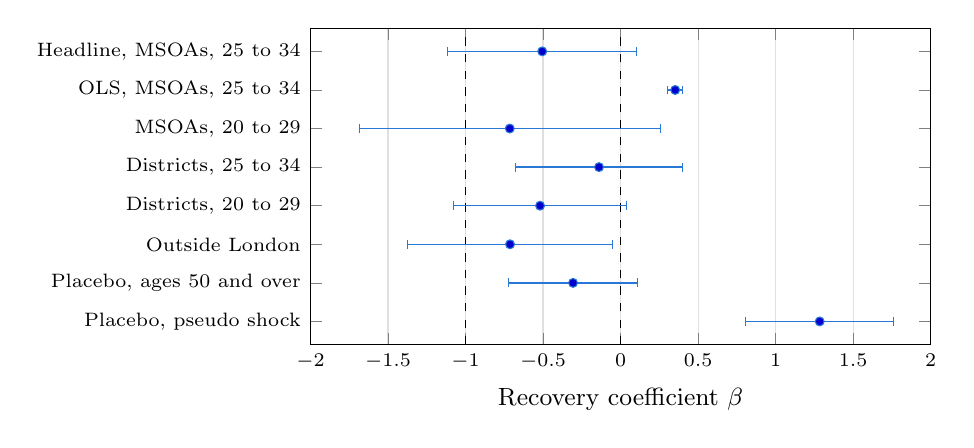
\begin{tikzpicture}
\begin{axis}[width=0.78\linewidth, height=5.6cm, xmin=-2, xmax=2, ymin=0.4, ymax=8.6,
  ytick={1,...,8}, yticklabels={{Placebo, pseudo shock},{Placebo, ages 50 and over},{Outside London},{Districts, 20 to 29},{Districts, 25 to 34},{MSOAs, 20 to 29},{OLS, MSOAs, 25 to 34},{Headline, MSOAs, 25 to 34}}, xmajorgrids, grid style={gray!25},
  tick label style={font=\scriptsize}, label style={font=\small},
  xlabel={Recovery coefficient $\beta$}]
\addplot[black, dashed, forget plot] coordinates {(-1,0.4) (-1,8.6)};
\addplot[black, dashed, forget plot] coordinates {(0,0.4) (0,8.6)};
\addplot+[only marks, color=cA, mark=*, mark size=1.6pt, error bars/x dir=both, error bars/x explicit,
  error bars/error bar style={line width=0.5pt, color=cA}] coordinates {(-0.5053,8) +- (0.6087,0) (0.3523,7) +- (0.0488,0) (-0.7146,6) +- (0.9719,0) (-0.1390,5) +- (0.5381,0) (-0.5193,4) +- (0.5578,0) (-0.7130,3) +- (0.6614,0) (-0.3065,2) +- (0.4181,0) (1.2844,1) +- (0.4779,0)};
\end{axis}
\end{tikzpicture}
\caption{Recovery coefficients from equation~(\ref{eq:rec}) with 95 per cent Wald intervals clustered by district. Dashed lines are drawn at full recovery, $-1$, and at a lasting shift, 0. District rows are for recovery to 2025 with region fixed effects. The headline minus the pseudo-shock coefficient is $-1.79$ (interval $-2.54$ to $-1.04$). London, with a first-stage F of 1.3, is omitted.}\label{fig:rec}
\end{figure}

\subsection{Registered tests and later choices}

To fix each verdict before its result was seen, the decision rules were written into three pre-analysis plans and fixed with SHA-256 checksums, namely the national plan, written before national estimation began, the venue-mix plan, written after the closure calendar and treatment diagnostics were built and before any outcome was opened, and the recovery plan, written after the population series were built and before any recovery regression. No departures were made from the venue-mix and recovery plans, and the London analyses preceded the plans and were not registered.

\begin{table}[htbp]
\centering
\caption{Registered tests, verdicts and further results}
\renewcommand{\arraystretch}{1.15}\label{tab:registered}
\footnotesize
\begin{tabularx}{\linewidth}{@{}>{\raggedright\arraybackslash}p{2.7cm}>{\raggedright\arraybackslash}p{3.5cm}>{\raggedright\arraybackslash}p{2.5cm}L@{}}
\toprule
Plan and test & Headline (p-value or interval) & Registered verdict & Further result \\
\midrule
National, triple difference & Reversal $-1.53$ (0.191) & Variety channel not supported & Young adults moved towards garden access in 2020, with an interaction of $+4.34$ ($<0.001$) \\
National, tier closures & Interaction $+0.24$ (0.847); first stage 0.581 & Uninformative & Within districts retail and recreation visits fell by 1.13 points per 10 extra closure days \\
National, Census small areas & $-6.18$ per SD of access ($<0.001$); placebo $+3.74$ (0.002) & Supported, with a mean-reversion caveat & Inflow rates rose faster from 2001 to 2011 where access was higher \\
National, rents & Deviation from trend $+0.15$ (0.569) & Null & Rents followed their pre-2020 trend through the closures \\
Venue mix & $-1.28$ per 10 days (0.011); placebo $+3.28$ ($<0.001$) & Not supported, placebo outside the rule & Local variety is mostly food and drink, and its loss correlates at $-0.92$ with the takeaway share \\
Recovery & $\beta = -0.51$ ($-1.11$ to $0.10$) & Inconclusive & Outside London $-0.71$ ($-1.37$ to $-0.05$), a reading of full recovery \\
\bottomrule
\end{tabularx}
\tabnote{Chosen after the registered results were known: the access and density measures, the density controls, the student-share checks and the deviations from the pre-2020 trend in Table~\ref{tab:ddd}. The headline minus pseudo-shock difference and the outside-London recovery coefficient were registered as further estimates outside the decision rule.}
\end{table}

\end{document}
